\documentclass[12pt,fleqn]{article}\usepackage{../../common}
\begin{document}
Boltzman Makinaları (Rasgele Hopfield Ağları) 

Alttaki ifade bir Boltmann dağılımını gösterir, 

$$  
P(x;W) = \frac{1}{Z(W)} 
\exp \bigg[ \frac{1}{2} x^T W x \bigg]
\mlabel{3}
$$

ki $x$ çok boyutlu ve -1,+1 değerleri içeren bir vektör, $W$ simetrik ve
çaprazında (diagonal) sıfır içeren bir matristir, $n \times d$ boyutlarındaki
bir veri için $d \times d$ boyutlarında olacaktır.  Boltzmann Makinaları (BM),
Kısıtlı Boltzmann Makinaları (Restricted Boltzmann Machines) kavramına geçiş
yapmadan önce iyi bir durak noktası.

BM $W$ içinde aslında tüm değişkenlerin ikisel ilişkisini içerir. $W$ çok
değişkenli Gaussian dağılımındaki $\Sigma$'da olduğu gibi ikisel bağlantıları
saptar. Veriden $W$'yu öğrenmek için olurluğu hesaplamak lazım. Olurluk
(likelihood)

$$  
\prod _{n=1}^{N} P(x^{(n)};W) = \frac{1}{Z(W)} 
\exp \bigg[ \frac{1}{2} x^{(n)^T} W x^{(n)} \bigg]
$$

Log olurluk

$$  
\mathcal{L} = \ln \big( \prod _{n=1}^{N} P(x^{(n)};W) \big) = 
\sum _{n=1}^{N} \bigg[ \frac{1}{2} x^{(n)^T} W x^{(n)} - \ln Z(W) \bigg]
\mlabel{1}
$$

Birazdan $\frac{\partial \mathcal L}{\partial w_{ij}}$ türevini alacağız, o
sırada $\ln Z(W)$'nin türevi lazım, daha doğrusu $Z(W)$'yi nasıl türevi alınır
hale getiririz?

$Z(W)$ normalizasyon sabiti olduğuna göre, dağılımın geri kalanının sonsuzlar
üzerinden entegrali (ya da toplamı) normalizasyon sabitine eşittir,

$$ 
Z(W) = \sum_x  \exp \bigg[ \frac{1}{2} x^T W x \bigg]
$$

$$ 
\ln Z(W) = \ln \bigg[ \sum_x  \exp \big( \frac{1}{2} x^T W x \big) \bigg]
$$

Log bazlı türev alınca log içindeki herşey olduğu gibi bölüme gider, ve log
içindekinin türevi alınırak bölüme koyulur. Fakat log içine dikkatli
bakarsak bu zaten $Z(W)$'nin tanımıdır, böylece denklemi temizleme şansı
doğdu, bölüme hemen $Z(W)$ deriz, ve türevi log'un içine uygularız,

$$ 
\frac{\partial}{\partial w_{ij}} \ln Z(W) = 
\frac{1}{Z(W)}
\bigg[ 
\sum_x \frac{\partial}{\partial w_{ij}} \exp \big( \frac{1}{2} x^T W x \big) 
\bigg]
$$

$$ 
\frac{\partial}{\partial w_{ij}} \exp \big( \frac{1}{2} x^T W x \big)  = 
\frac{1}{2}  \exp \big( \frac{1}{2} x^T W x \big) 
\frac{\partial}{\partial w_{ij}}x^T W x
\mlabel{2}
$$

(2)'in içindeki bölümü açalım,

$$ 
\frac{\partial}{\partial w_{ij}}x^T W x = x_i x_j 
$$

Şimdi (2)'ye geri koyalım,

$$ 
= \frac{1}{2} \exp \big( \frac{1}{2} x^T W x \big) x_i x_j
$$

$$ 
\frac{\partial}{\partial w_{ij}} \ln Z(W) = 
\frac{1}{Z(W)}
\bigg[ 
\sum_x \frac{1}{2}  \exp \big( \frac{1}{2} x^T W x \big) x_i x_j
\bigg]
$$

$$ 
= \frac{1}{2} \sum_x 
\frac{1}{Z(W)} \exp \big( \frac{1}{2} x^T W x \big) x_i x_j 
$$

$$ 
= \frac{1}{2}  \sum_x P(x;W) x_i x_j
$$

Üstteki son ifadede bir kısaltma kullanalım,

$$ 
\sum_x P(x;W) x_i x_j =  < x_i,x_j >_{P(x;W)}
\mlabel{4}
$$

Artık $\ln Z(W)$'nin türevini biliyoruz. O zaman tüm log olurluğun türevine
(1) dönebiliriz, 

$$  
\frac{\partial \mathcal{L}}{\partial w_{ij}} = 
\sum _{n=1}^{N} \bigg[ 
\frac{\partial}{\partial w_{ij}}  \frac{1}{2} x^{(n)^T} W x^{(n)} - 
\frac{\partial}{\partial w_{ij}}  \ln Z(W) \bigg]
$$

$$  
= \sum_{n=1}^{N} 
\bigg[ 
\frac{1}{2} x_i^{(n)^T}x_j^{(n)} - 
\frac{\partial}{\partial w_{ij}}  \ln Z(W) 
\bigg]
$$

$$  
= \sum _{n=1}^{N} 
\bigg[ 
\frac{1}{2} x_i^{(n)^T}x_j^{(n)} - 
\frac{1}{2}< x_i x_j >_{P(x;W)}
\bigg]
$$ 

1/2 sabitlerini atalım, 

$$  
= \sum _{n=1}^{N} 
\bigg[ 
 x_i^{(n)^T}x_j^{(n)} - < x_i x_j >_{P(x;W)}
\bigg]
$$

Eğer 

$$
< x_i x_j >_{Data} = \frac{1}{N} \sum _{n=1}^{N}  x_i^{(n)^T}x_j^{(n)}
$$

olarak alırsak, eşitliğin sağ tarafı verisel kovaryansı (empirical
covariance) temsil eder. Düzenleyince,

$$ 
N \cdot < x_i x_j >_{Data} = \sum _{n=1}^{N}  x_i^{(n)^T}x_j^{(n)}
$$

şimdi eşitliğin sağ tarafı üç üstteki formüle geri koyulabilir,

$$ 
\frac{\partial \mathcal{L}}{\partial w_{ij}}  = 
N \big[ < x_i x_j >_{Data}  - < x_ix_j >_{P(x;W)} \big] 
$$

Her ne kadar $N$ veri noktası sayısını gösteriyor olsa da, üstteki ifade
bir gradyan güncelleme formülü olarak ta görülebilir, ve $N$ yerine bir
güncelleme sabiti alınabilir. Gradyan güncelleme olarak görülebilir çünkü
$w_{ij}$'ye göre türev aldık, o zaman bizi $\mathcal{L}$'in minimumuna götürecek
$w$ adımları üstte görüldüğü gibidir. 

(4)'te görülen $< x_ix_j >_{P(x;W)}$'in anlamı nedir? Bu ifade mümkün tüm $x$
değerleri üzerinden alınıyor ve ikisel ilişkilerin olasılığını ``mevcut
modele'' göre hesaplıyor. Yani bu ifade de bir korelasyon hesabıdır, sadece
veriye göre değil, tüm mümkün değerler ve model üzerinden alınır. Bu hesabı
yapmak oldukça zordur, fakat yaklaşıksal olarak Monte Carlo yöntemi ile
hesaplanabilir. Nihayet MC ve MCMC metotlarının kullanılma sebebini görmeye
başlıyoruz; bu metotlar zaten aşırı yüksek boyutlu, analitik çözümü
olmayan, hesaplanamaz (intractable) entegraller (ya da toplamlar) için
keşfedilmiştir. 

Yani bu ifadeyi hesaplamak için Monte Carlo simulasyonu kullanacağız. Tüm
değerleri teker teker ziyaret etmek yerine (ki bu çok uzun zaman alırdı)
mevcut modele en olası $x$ değerleri ``ürettireceğiz'', ve bu değerleri
alıp sanki gerçek veriymiş gibi sayısal korelasyonlarını
hesaplayacağız. Eğer veriler dağılımın en olası noktalarından geliyorlarsa,
elimizde veri dağılımı ``iyi'' temsil eden bir veri setidir. Daha sonra bu
korelasyon hesabını değeri gerçek veri korelasyonunundan çıkartıp bir sabit
üzerinden gradyan adımı atmamız mümkün olacak.

Gibbs Örneklemesi (Sampling)

Gibbs örneklemesinin detayları için [5]. Bolzmann dağılımından örneklem
almak için bize tek bir değişken (hücre) haricinde diğer hepsinin bilindiği
durumun olasılık hesabı lazım, yani koşulsal olasılık
$P(x_i = 1 | x_j, j \ne i)$. Yani $x$ üzerinde, biri hariç tüm öğelerin
bilindiği durumda bilinmeyen tek hücre $i$'nin 1 olma olasılık değeri,

$$ 
P(x_i = 1 | x_j, j \ne i) = \frac{1}{1 + e^{-a_i}} 
$$

ve,

$$ 
a_i = \sum_j  w_{ij}x_j 
$$

Bu koşulsal olasılığın temiz / basit bir formül olması önemli, üstteki
görülen bir sigmoid fonksiyonu bu türden bir fonksiyondur... Bu
fonksiyonlar hakkında daha fazla bilgi [6] yazısında bulunabilir.

Ama, ana formül (3)'ten bu noktaya nasıl eriştik? Bu noktada biraz türetme
yapmak lazım. $x$ vektörü içinde sadece $x_i$ öğesinin $b$ olmasını $x^b$ olarak
alalım. Önce koşulsal dağılımda ``verili'' olan kısmı elde etmek lazım. O
uzaman

$$ 
P(x_j,j \ne i) = P(x^0) + P(x^1) 
$$

Bu bir marjinalizasyon ifadesi, tüm olası $i$ değerleri üzerinde bir toplam
alınca geri kalan $j$ değerlerinin dağılımını elde etmiş oluruz. 

$$  
P(x_i = 1 | x_j,j \ne i)  = \frac{P(x^1)}{P(x^0) + P(x^1)} 
$$

çünkü $P(A|B) = P(A,B) / P(B)$ bilindiği gibi, ve $P(x^1)$ içinde $x_1=1$
setini içeren tüm veriler üzerinden. 

Eşitliğin sağ tarafında $P(x^1)$'i bölen olarak görmek daha iyi, ayrıca
ulaşmak istediğimiz $1/1 + e^{-a_i}$ ifadesinde $+1$'den kurtulmak iyi
olur, böylece sadece $e^{-a_i}$ olan eşitliği ispatlarız. Bunun her iki
denklemde ters çevirip 1 çıkartabiliriz,

$$  
1 / P(x_i = 1 | x_j,j \ne i) = \frac{P(x^0) + P(x^1)}{P(x^1)} 
$$

$$
= 1 + \frac{ P(x^0)}{P(x^1)}
$$

Bir çıkartırsak, $\frac{ P(x^0)}{P(x^1)}$ kalır. Bu bize ulaşmak
istediğimiz denklemde $e^{-a_i}$ ibaresini bırakır. Artık sadece
$\frac{P(x^0)}{P(x^1)}$'in $e^{-a_i}$'e eşit olduğunu göstermek yeterli.


$$ 
\frac{ P(x^0)}{P(x^1)} = \exp( x^{0^T}Wx^0 -   x^{1^T}Wx^1 )
$$

Şimdi $x^TWx$ gibi bir ifadeyi indisler bazında açmak için şunları yapalım, 

$$ 
x^TWx = \sum_{k,j} x_kx_jw_{kj} 
$$

Üstteki çok iyi bilinen bir açılım. Eğer

$$ 
\sum_{k,j} \underbrace{x_kx_jw_{ij}}_{Y_{kj}} = \sum_{k,j}Y_{kj} 
$$

alırsak birazdan yapacağımız işlemler daha iyi görülebilir. Mesela $k=i$
olan durumu dış toplamdan dışarı çekebiliriz

$$ 
= \sum_{k \ne i}\sum_j Y_{kj} + \sum_{j} Y_{ij}
$$

Daha sonra $j = i$ olan durumu iç toplamdan dışarı çekebiliriz, 

$$ 
= \sum_{k \ne i}( \sum_{j \ne i} Y_{kj} + Y_{ki}) + \sum_{j} Y_{ij}
$$

İç dış toplamları birleştirelim,

$$ 
= \sum_{k \ne i,j \ne i} Y_{kj} + \sum_{k \ne i}  Y_{ki} + \sum_{j} Y_{ij}
$$

$$ 
= \sum_{k \ne i,j \ne i} Y_{kj} + \sum_{k}  Y_{ki} + \sum_{j} Y_{ij} + Y_{ii}
$$

Üstteki ifadeyi $ \exp( x^{0^T}Wx^0 -   x^{1^T}Wx^1 )$ için kullanırsak,

$$ 
\exp 
\big( 
\sum_{k}  Y_{ki}^0 + \sum_{j} Y_{ij}^0 + Y_{ii}^0 - 
( \sum_{k}  Y_{ki}^1 + \sum_{j} Y_{ij}^1 + Y_{ii}^1  )
\big)
$$

$\sum_{k \ne i,j \ne i} Y_{kj}$ teriminin nereye gittiği merak edilirse,
bu ifade $i$'ye dayanmadığı için bir eksi bir artı olarak iki defa dahil
edilip iptal olacaktı. 

$$ 
= \exp \big( 
0 - ( \sum_{k}  Y_{ki}^1 + \sum_{j} Y_{ij}^1 + Y_{ii}^1  ) 
\big)
$$

$W$'nin simetrik matris olduğunu düşünürsek, $\sum_{k}  Y_{ki}^1$ ile 
$\sum_{j}Y_{ij}^1$ aynı ifadedir, 

$$ 
= \exp \big( 
- ( 2 \sum_{j} Y_{ij}^1 + Y_{ii}^1  ) 
\big)
$$

$W$ sıfır çaprazlı bir matristir, o zaman $Y_{ii}^1=0$, 

$$ 
= \exp \big( 2 \sum_{j} Y_{ij}^1 \big) = \exp (- 2 a_i )
$$

Orijinal dağılım denkleminde $1/2$ ifadesi vardı, onu başta işlemlere dahil
etmemiştik, edilseydi sonuç  $\exp (- a_i)$ olacaktı. 

\inputminted[fontsize=\footnotesize]{python}{boltz.py}

Fonksiyon \verb!draw! içinde, tek bir veri satırı için ve sırayla her
değişken (hücre) için, diğer değişkenleri baz alıp diğerinin koşulsal
olasılığını hesaplıyoruz, ve sonra bu olasılığı kullanarak bir sayı üretimi
yapıyoruz. Üretimin yapılması için \verb!np.random.rand!'dan gelen 0 ve 1
arasındaki birörnek (uniform) dağılımdan bir rasgele sayıyı geçip geçmeme
irdelemesi yeterli. Bir Bernoulli olasılık hesabını üretilen bir rasgele
değişkene bu şekilde çevirebilirsiniz. Bu niye işler? Üstte belirttiğimiz
irdelemeyi rasgele değişken olarak kodlarsak (ki bu da bir Bernoulli
rasgele değişkeni olur), ve birörnek rasgele değişken $U$ olsun,

$$ Y = 
\left\{ \begin{array}{ll}
1 & U < p \\
0 & U \ge p \\
\end{array} \right.
$$

Bu durumda $P(X=1) = P(U<p) = p$ olurdu. Neden? Çünkü üstte bir sürekli
(continuous) bir birörnek değişken yarattık, ve $P(U<p) = F_u(p) = p$.

Devam edelim; Çağrı \verb!sample! ise \verb!draw!'u kullanarak pek çok veri
satırını içeren ve dağılımı temsil eden bir örneklem yaratmakla
sorumlu. Bunu her örneklem satırını baz alarak bir sonrakini ürettirerek
yapıyor, böylelikle MCMC'nin dağılımı ``gezmesi'' sağlanmış oluyor.

Normalizasyon Sabiti

Birazdan göreceğimiz örnek için normalizasyon sabitini de hesaplamamız
gerekecek. Niye? Mesela iki farklı BM dağılımını farklı etiketli verilerden
öğreniyoruz, sonra test veri noktasını her iki ayrı dağılıma ``soruyoruz''?
Olasılığı nedir? Bu noktada kesin bir olasılık hesabı istediğimiz için
artık $Z$ bilinmek zorunda. Bu sabitin hesaplanması için ise
$< x_ix_j >_{P(x;W)}$ için olduğu gibi, tüm mümkün $x$'ler üzerinden bir
toplam gerekir, bu toplam $\sum_x \exp 1/2 x^T W x$ toplamı. Bu toplamın
hesaplanması çok zor olduğu için, yine MCMC'ye başvuracağız. Tek fark
alınan örneklemi (3) formülüne geceğiz, ve bir olasılık hesabı yapacağız,
ve bu olasılıkları toplayacağız. Tabii aynı $x$'i (eğer tekrar tekrar
üretilirse -ufak bir ihtimal ama mümkün-) tekrar tekrar toplamamak için
hangi $x$'lerin üretildiğini bir sözlük içinde hatırlayacağız, yani bir $x$
olasılığı sadece bir kere toplanacak.

Şimdi ufak bir örnek üzerinde BM'i işletelim. 

\begin{minted}[fontsize=\footnotesize]{python}
import boltz
A = np.array([\
[0.,1.,1.,1],
[1.,0.,0,0],
[1.,1.,1.,0],
[0, 1.,1.,1.],
[1, 0, 1.,0]
])
A[A==0]=-1

clf = boltz.Boltzmann(n_iter=50,eta=0.01,sample_size=200,init_sample_size=50)
clf.fit(A)
print 'W'
print clf.W
print 'normalizasyon sabiti', clf.C
\end{minted}

\begin{verbatim}
Iteration 0
Iteration 10
Iteration 20
Iteration 30
Iteration 40
W
[[ 0.    -0.065 -0.06  -0.055]
 [-0.065  0.     0.17   0.105]
 [-0.06   0.17   0.    -0.09 ]
 [-0.055  0.105 -0.09   0.   ]]
normalizasyon sabiti 16.4620358997
\end{verbatim}

Sonuç $W$ üstte görüldüğü gibi. Örnek veriye bakarsak 2. satır 3. kolonda
artı bir değer var, 1. satır 4. kolonda eksi değer var. Bu beklediğimiz bir
şey çünkü 2. ve 3. değişkenlerin arasında bir korelasyon var, $x_2$ ne
zaman 1/0 ise $x_3$ te 1/0. Fakat $x_1$ ile $x_4$ ters bir korelasyon var,
birbirlerinin zıttı değerlere sahipler. 

Şimdi yeni test verisini dağılıma ``soralım'', 

\begin{minted}[fontsize=\footnotesize]{python}
test = np.array([\
[0.,1.,1.,1],
[1.,1.,0,0],
[0.,1.,1.,1]
])    
print clf.predict_proba(test)
\end{minted}

\begin{verbatim}
[ 0.0730905   0.05692294  0.0730905 ]
\end{verbatim}

Görüntü Tanıma

Elimizde el yazısı tanıma algoritmaları için kullanılan bir veri seti var.
Veride 0,5,7 harflerinin görüntüleri var. Mesela 5 için bazı örnek
görüntüler,

\begin{minted}[fontsize=\footnotesize]{python}
Y = np.loadtxt('../../stat/stat_mixbern/binarydigits.txt')
label = np.ravel(np.loadtxt('../../stat/stat_mixbern/bindigitlabels.txt'))
Y5 = Y[label==5]
plt.imshow(Y5[0,:].reshape((8,8),order='C'), cmap=plt.cm.gray)
plt.savefig('boltzmann_01.png')

plt.imshow(Y5[1,:].reshape((8,8),order='C'), cmap=plt.cm.gray)
plt.savefig('boltzmann_02.png')

plt.imshow(Y5[2,:].reshape((8,8),order='C'), cmap=plt.cm.gray)
plt.savefig('boltzmann_03.png')
\end{minted}

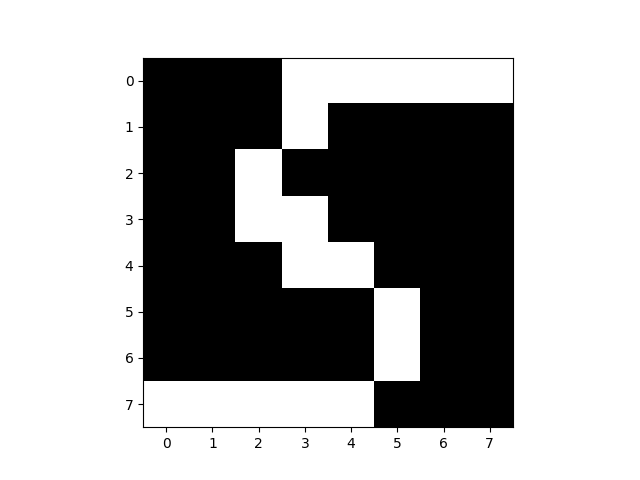
\includegraphics[height=3cm]{boltzmann_01.png}
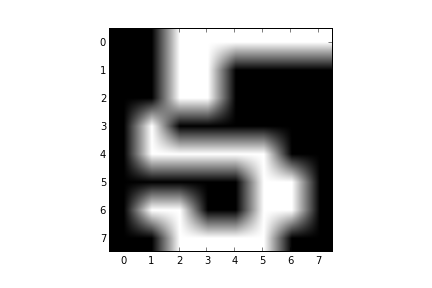
\includegraphics[height=3cm]{boltzmann_02.png}
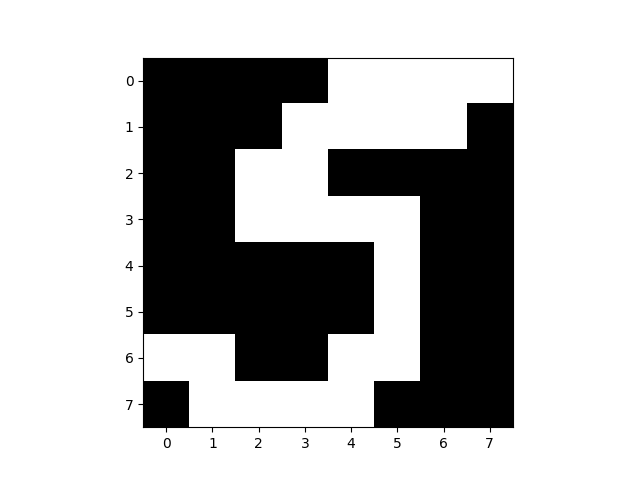
\includegraphics[height=3cm]{boltzmann_03.png}

Bu görüntüleri tanımak için BM kullanalım. Eğitim ve test olarak veriyi
ikiye ayıracağız, ve eğitim seti her etiketin $W$'sini öğrenmek için
kullanılacak. Daha sonra test setinde her veri noktalarını her üç BM'ye
ayrı ayrı ``sorup'' o test verisinin o BM'e göre olasılığını alacağız, ve
hangi BM daha yüksek olasılık döndürüyorsa etiket olarak onu kabul
edeceğiz. Hangi BM daha yüksek olasılık döndürüyorsa, o BM ``bu verinin
benden gelme olasılığı yüksek'' diyor demektir, ve etiket o olmalıdır.

\inputminted[fontsize=\footnotesize]{python}{testbm.py}

\begin{minted}[fontsize=\footnotesize]{python}
!python testbm.py
\end{minted}

\begin{verbatim}
Iteration 0
Iteration 10
Iteration 20
Iteration 0
Iteration 10
Iteration 20
Iteration 0
Iteration 10
Iteration 20
Boltzmann Makinasi 0.975
KNN 0.975
\end{verbatim}

Sonuç yüzde 97.5, oldukça yüksek, ve KNN metotu ile aynı sonucu aldık, ki
bu aslında oldukça temiz / basit bir veri seti için fena değil.

Biraz Hikaye

Boltzman Makinalarıyla ilgilenmemizin ilginç bir hikayesi var. Aslında bu
metottan haberimiz yoktu, ayrıca mevcut işimizde 0/1 içeren ikisel
verilerle çok hasır neşirdik, ve bu tür verilerde ikisel ilişkiler
(coöccürence) hesabı iyi sonuçlar verir, ki bu hesap basit bir matris
çarpımı ile elde edilir.

\begin{minted}[fontsize=\footnotesize]{python}
import numpy as np
A = np.array([\
[0.,1.,1.,0],
[1.,1.,0, 0],
[1.,1.,1.,0],
[0, 1.,1.,1.],
[0, 0, 1.,0]
])
c = A.T.dot(A).astype(float)
print c 
\end{minted}

\begin{verbatim}
[[ 2.  2.  1.  0.]
 [ 2.  4.  3.  1.]
 [ 1.  3.  4.  1.]
 [ 0.  1.  1.  1.]]
\end{verbatim}

Burada bakılırsa 2. satır 3. kolon 3 değerini taşıyor çünkü 2. ve
3. değişkenlerin aynı anda 1 olma sayısı tam olarak 3. Sonra acaba bu
bilgiyi veri üzerinde hesaplayıp bir kenara koysak bir dağılım gibi
kullanamaz mıyız, sonra yeni veri noktasını bu ``dağılıma sorabiliriz''
diye düşündük. Biraz matris çarpım cambazlığı sonrası, yeni veri noktası
için

\begin{minted}[fontsize=\footnotesize]{python}
x = np.array([0,1,1,0])
print np.dot(np.dot(x.T,c), x) / 2
\end{minted}

\begin{verbatim}
7.0
\end{verbatim}

gibi sonuçlar alabildiğimizi gördük; Bu değerin ilişki matrisinin tam
ortasındaki 4,3,3,4 sayılarının toplamının yarısı olduğuna dikkat
edelim. Yani $x$ çarpımı ilişki matrisinin sadece kendini ilgilendiren
kısmını çekip çıkarttı, yani 2. ve 3. değişenleri arasındaki ilişkiyi
toplayıp aldı.

Buradan sonra, ``acaba bu bir dağılım olsa normalizasyon sabiti ne
olurdu?'' sorusuna geldik, ki [4] sorusu buradan çıktı ve bu soruya bomba
bir cevap geldi. Sonra diğer okumalarımız sırasında Boltzmann Dağılımına
ulaştık, bu dağılımın ek olarak bir $\exp$ tanımı var (ki türev alımı
sırasında bu faydalı), ve tabii öğrenim için daha net bir matematiği
var. Biz de maksimum olurluk ile [4]'teki fikrin sayısal kovaryansa
ulaştırıp ulaştırmayacağını merak ediyorduk, BM formunda verisel kovaryans
direk elde ediliyor. Böylece BM konusuna girmiş olduk. 

Bitirmeden önce ufak not, BM'ler Kısıtlı BM (RBM) için bir zıplama tahtası,
ve RBM'ler Derin Öğrenimin (Deep Learning) bir türü için kullanılabilir, bu
yapay sinir ağlarını birden fazla RBM'leri üst üste koyarak elde etmek
mümkün (gerçi son zamanlarda moda yaklaşım evrişimsel ağ -convolutional
network- kullanmak).

[1] D. MacKay, {\em Information Theory, Inference and Learning Algorithms}, sf. 523

[2] Flaxman, {\em Notebook}, \url{http://nbviewer.ipython.org/gist/aflaxman/7d946762ee99daf739f1}

[3] Stack Exchange, {\em From $P(x;W) = \frac{1}{Z(W)} \exp \bigl[ \frac{1}{2} x^T W x
  \bigr]$ to Sigmoid}, \url{http://math.stackexchange.com/questions/1095491/from-pxw-frac1zw-exp-bigl-frac12-xt-w-x-bigr-to-sigmoid/}

[4] Stack Exchange, {\em Calculating the sum $\frac{1}{2} \sum x^T \Sigma x$ for all $x \in
  \{0,1\}^n$}, \url{http://math.stackexchange.com/questions/1080504/calculating-the-sum-frac12-sum-xt-sigma-x-for-all-x-in-0-1-n}

[5] Bayramli, Istatistik, {\em Monte Carlo, Entegraller, MCMC}

[6] Bayramli, Istatistik, {\em Lojistik Regresyon}

\end{document}
